%%%%%%%%%%%%%%%%%%%%%%%%%%%%%%%%%%%%%%%%%
\documentclass{article} % 'openany' here removes the gap page between days, erase it to restore this gap; 'oneside' can also be added to remove the shift that odd pages have to the right for easier reading

\usepackage[margin=1.00in]{geometry}

\usepackage[ 
  backref=page,
  pdfpagelabels=true,
  plainpages=false,
  colorlinks=true,
  bookmarks=true,
  pdfview=FitB]{hyperref} % Required for the hyperlinks within the PDF
  
\usepackage{booktabs} % Required for the top and bottom rules in the table
\usepackage{float} % Required for specifying the exact location of a figure or table
\usepackage{graphicx} % Required for including images2
\usepackage{lipsum} % Used for inserting dummy 'Lorem ipsum' text into the template
\usepackage{subfigure}
\newcommand{\HRule}{\rule{\linewidth}{0.5mm}} % Command to make the lines in the title page
\setlength\parindent{0pt} % Removes all indentation from paragraphs



%---------------------------------------------------------------------------------------
%%% TO ADD MATLAB FILES %%%%%
\usepackage{listings}
\lstset{basicstyle=\ttfamily\footnotesize,breaklines=true}
\usepackage{color} %red, green, blue, yellow, cyan, magenta, black, white
\definecolor{mygreen}{RGB}{28,172,0} % color values Red, Green, Blue
\definecolor{mylilas}{RGB}{170,55,241}
%%%%%%%%%%%%%%%%%%%%%%%%%%%%%
\usepackage{wrapfig}
\begin{document}

% ---------------- TO ADD MATLAB FILES --------
\lstset{language=Matlab,%
    %basicstyle=\color{red},
    breaklines=true,%
    morekeywords={matlab2tikz},
    keywordstyle=\color{blue},%
    morekeywords=[2]{1}, keywordstyle=[2]{\color{black}},
    identifierstyle=\color{black},%
    stringstyle=\color{mylilas},
    commentstyle=\color{mygreen},%
    showstringspaces=false,%without this there will be a symbol in the places where there is a space
    numbers=left,%
    numberstyle={\tiny \color{black}},% size of the numbers
    numbersep=9pt, % this defines how far the numbers are from the text
    emph=[1]{for,end,break},emphstyle=[1]\color{red}, %some words to emphasise
    %emph=[2]{word1,word2}, emphstyle=[2]{style},    
}
%%%%%%%%%%%%%%%%%%%%%%%%%%%%%%%%%%%%%%%%%%%%%%%

%----------------------------------------------------------------------------------------
%	TITLE PAGE
%----------------------------------------------------------------------------------------

%\frontmatter % Use Roman numerals for page numbers
\title{
\begin{center}
\HRule \\[0.4cm]
{\Huge \bfseries Experiment 3: Acceleration during Pendulum Motion \\[0.5cm] \Large ME-330}\\[0.4cm] % Degree
\HRule \\[1.5cm]
\end{center}
}
\author{\Huge Dr. Vibahv Durgesh \\ \\ \LARGE vdurgesh@uidaho.edu \\[2cm]} % Your name and email address
\date{Week-02} % Beginning date
\maketitle

\tableofcontents

\clearpage



\section{Learning objective}
The objectives of this experiment are to provide the student with an opportunity to:

\begin{itemize}
\item Gain additional experience with Matlab.
\item Create a simple program for data acquisition using toolbox and National Instrument’s USB-6001.
\item Become familiar with breadboards, digital power supply, wiring, digital multi-meters, and other
laboratory skills.
\item Perform calibration of a MEMS accelerometer and create the calibration plot.
\item Compare measured normal acceleration to acceleration calculated from angular velocity during
fixed axis rotation.
\end{itemize}

\section{Equipment checklist}
\begin{itemize}
\item USB Data Acquisition Device (NI USB-6001).
\item Pendulum with Potentiometer (10$k\Omega$ Bourns 6639s) pivot and end-mounted accelerometer (MMA7361LC).
\item Needle nose pliers \& wire strippers. 
\item Breadboard – JE25
\item Small flathead screwdriver.
\item Digital multi-meter (DMM)
\item Power supply and wire kit.
\end{itemize}

\section{Introduction}
\begin{wrapfigure}{r}{0.35\textwidth}

\includegraphics[width=2.20in]{Fig01.png}
\caption{Schematic of the experimental setup.}
\label{fig:01}
\end{wrapfigure}
During rotation about a fixed axis, the normal acceleration of a point can be calculated from the angular velocity of the rotation motion according to the following formula:
\begin{equation}
a_{n} = -\dot{\theta}^2 r
\label{Eq:NormAcc}
\end{equation}


\section{Laboratory instruction}
This experiment will build on your work from the previous week. In addition to measuring the pendulum angle with a calibrated potentiometer, you will also measure normal acceleration of the end of the pendulum using a MEMS accelerometer. Schematic is shown in figure \ref{fig:01}. Start by setting up the NI USB-6001 to acquire data from the potentiometer and accelerometer. Next, you will calibrate the y-axis of the accelerometer. Finally, we will compare measured normal acceleration of the pendulum end to normal acceleration calculated from the derivative of the pendulum angle.
\section{Part-A}
Creating data acquisition program using Matlab data acquisition toolbox\\
A sample Matlab program is provided in the appendix section of the instruction use that program as the starting point and modify accordingly. The modified Matlab data acquisition program should acquire data from two-channels of the NI-DAQ, display and record the data.
\begin{itemize}
\item Make sure that matlab program is acquiring data from two channels, The first channel should be acquiring  potentiometer angle data and the second channel is acquiring the MEMS accelerometer data
\begin{itemize}
\item For Input Range, use $\pm$10 Volts for the potentiometer and $\pm$10 Volts for the accelerometer.
\item Set the sample rate to 1000 samples/sec. We will be calculating a discrete derivative of the
pendulum angle and a higher sample rate will reduce the noise from the process.
\end{itemize}
\item  The plot should be displaying the voltages from the accelerometer y-axis. You will need these for calibration of accelerometer.
\item Please use the calibration equation from the previous laboratory experiment. If in doubt please contact the TAs for the correct calibration. The calibration should be able to convert the potentiometer output voltage
to radians. Program this equation into the Matlab acquisition program. Verify that the calibration is producing the correct output by moving the pendulum to several known angles.
\item Measure the length of the pendulum are from Pivot point to accelerometer location. This will be used to calculate acceleration from angular position data.
\end{itemize}

\section{Part-B}
Connect the y-axis accelerometer output to the data acquisition using a breadboard. 
\begin{wrapfigure}{r}{0.35\textwidth}

\includegraphics[width=2.20in, angle=-90,origin=c]{Fig02.png}
\caption{The MMA7361LC 3-axis accelerometer with voltage regulator.}
\label{fig:02}
\end{wrapfigure}
\begin{itemize}
\item For this experiment, a 3-axis accelerometer has been fixed to the end of the pendulum apparatus (see Figure \ref{fig:02}). The accelerometer has been configured for $\pm$6g operation. The y- axis of the pendulum points towards the pendulum rotation axis (see Figure 3). For more information about the accelerometer, see \href{https://www.pololu.com/product/1251}{Pololu}.
\item Connect the accelerometer to the breadboard using the provided 3-wire cable. See figure \ref{fig:fig03A}.
\item Connect the Vin and GND pins on the accelerometer to the 5 Volt supply power (already used to power the potentiometer). See figure \ref{fig:fig03B} for reference.
\item Connect the y-axis accelerometer output to AI1 (Differential Analog Input 1). See figure \ref{fig:fig03C}.
\item Connect the DAQ GND, instead of the AI1-, to the ground on the breadboard. See figure \ref{fig:fig03C}.
\end{itemize}
\begin{figure}[!htb]
\centering
\subfigure[Sample connection to the accelerometer.]{%
\label{fig:fig03A}%
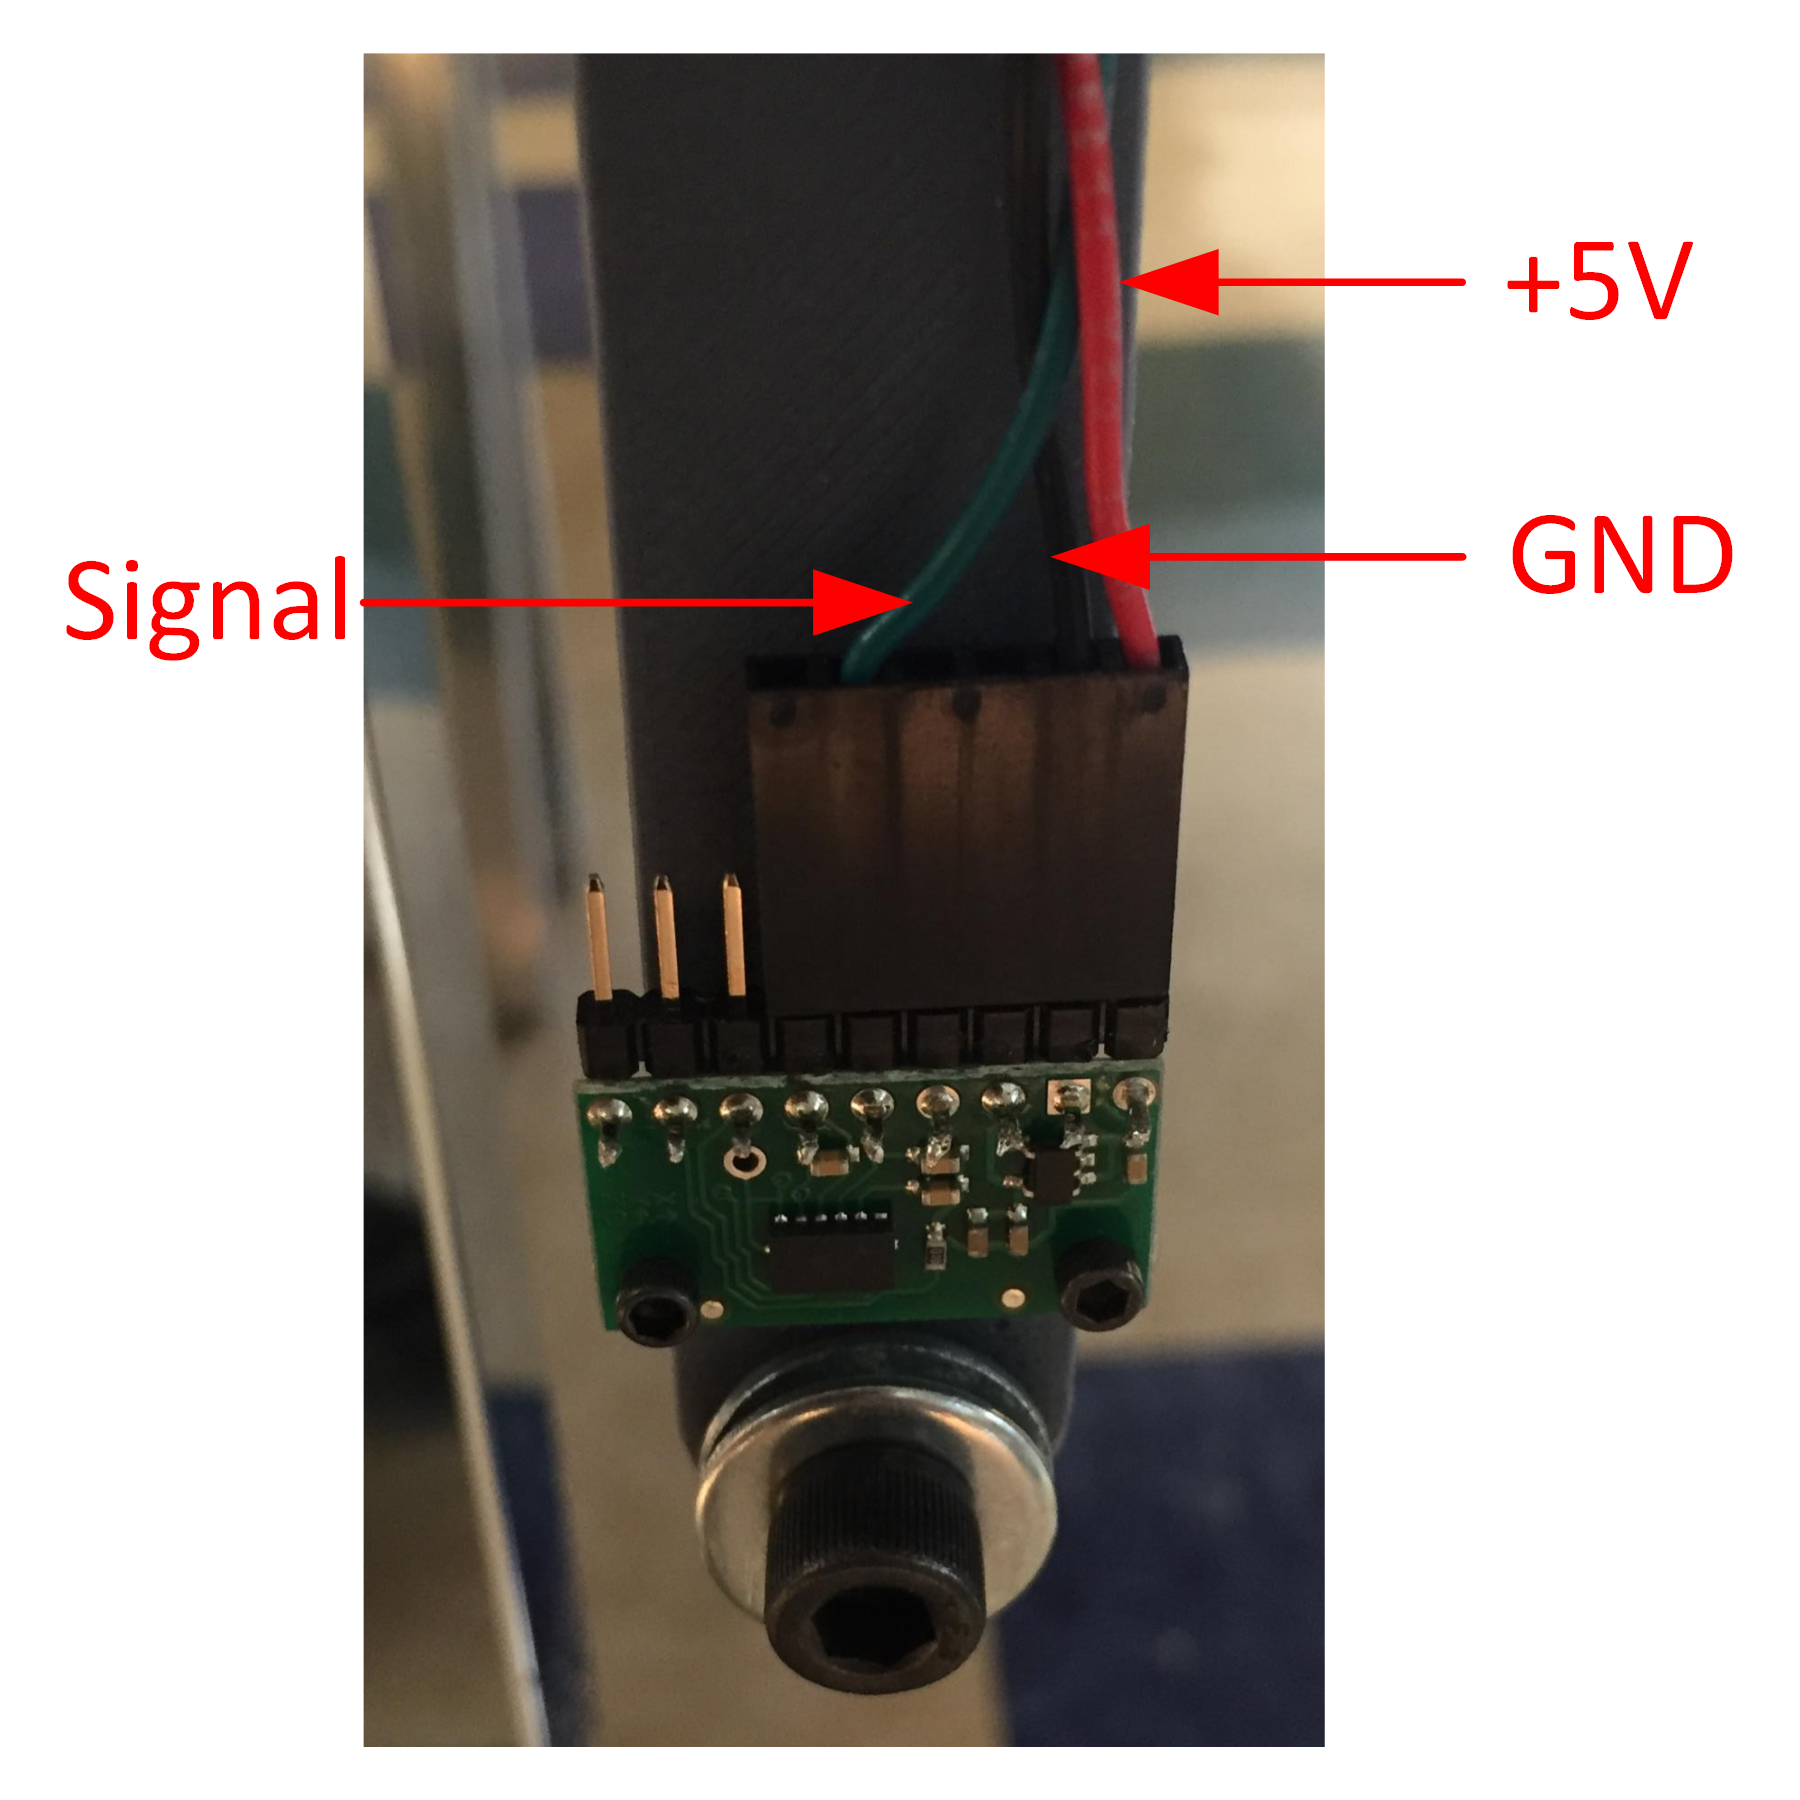
\includegraphics[width=2.75in]{Lab03Fig01.png}}%
\qquad
\subfigure[Sample connection to the accelerometer.]{%
\label{fig:fig03B}%
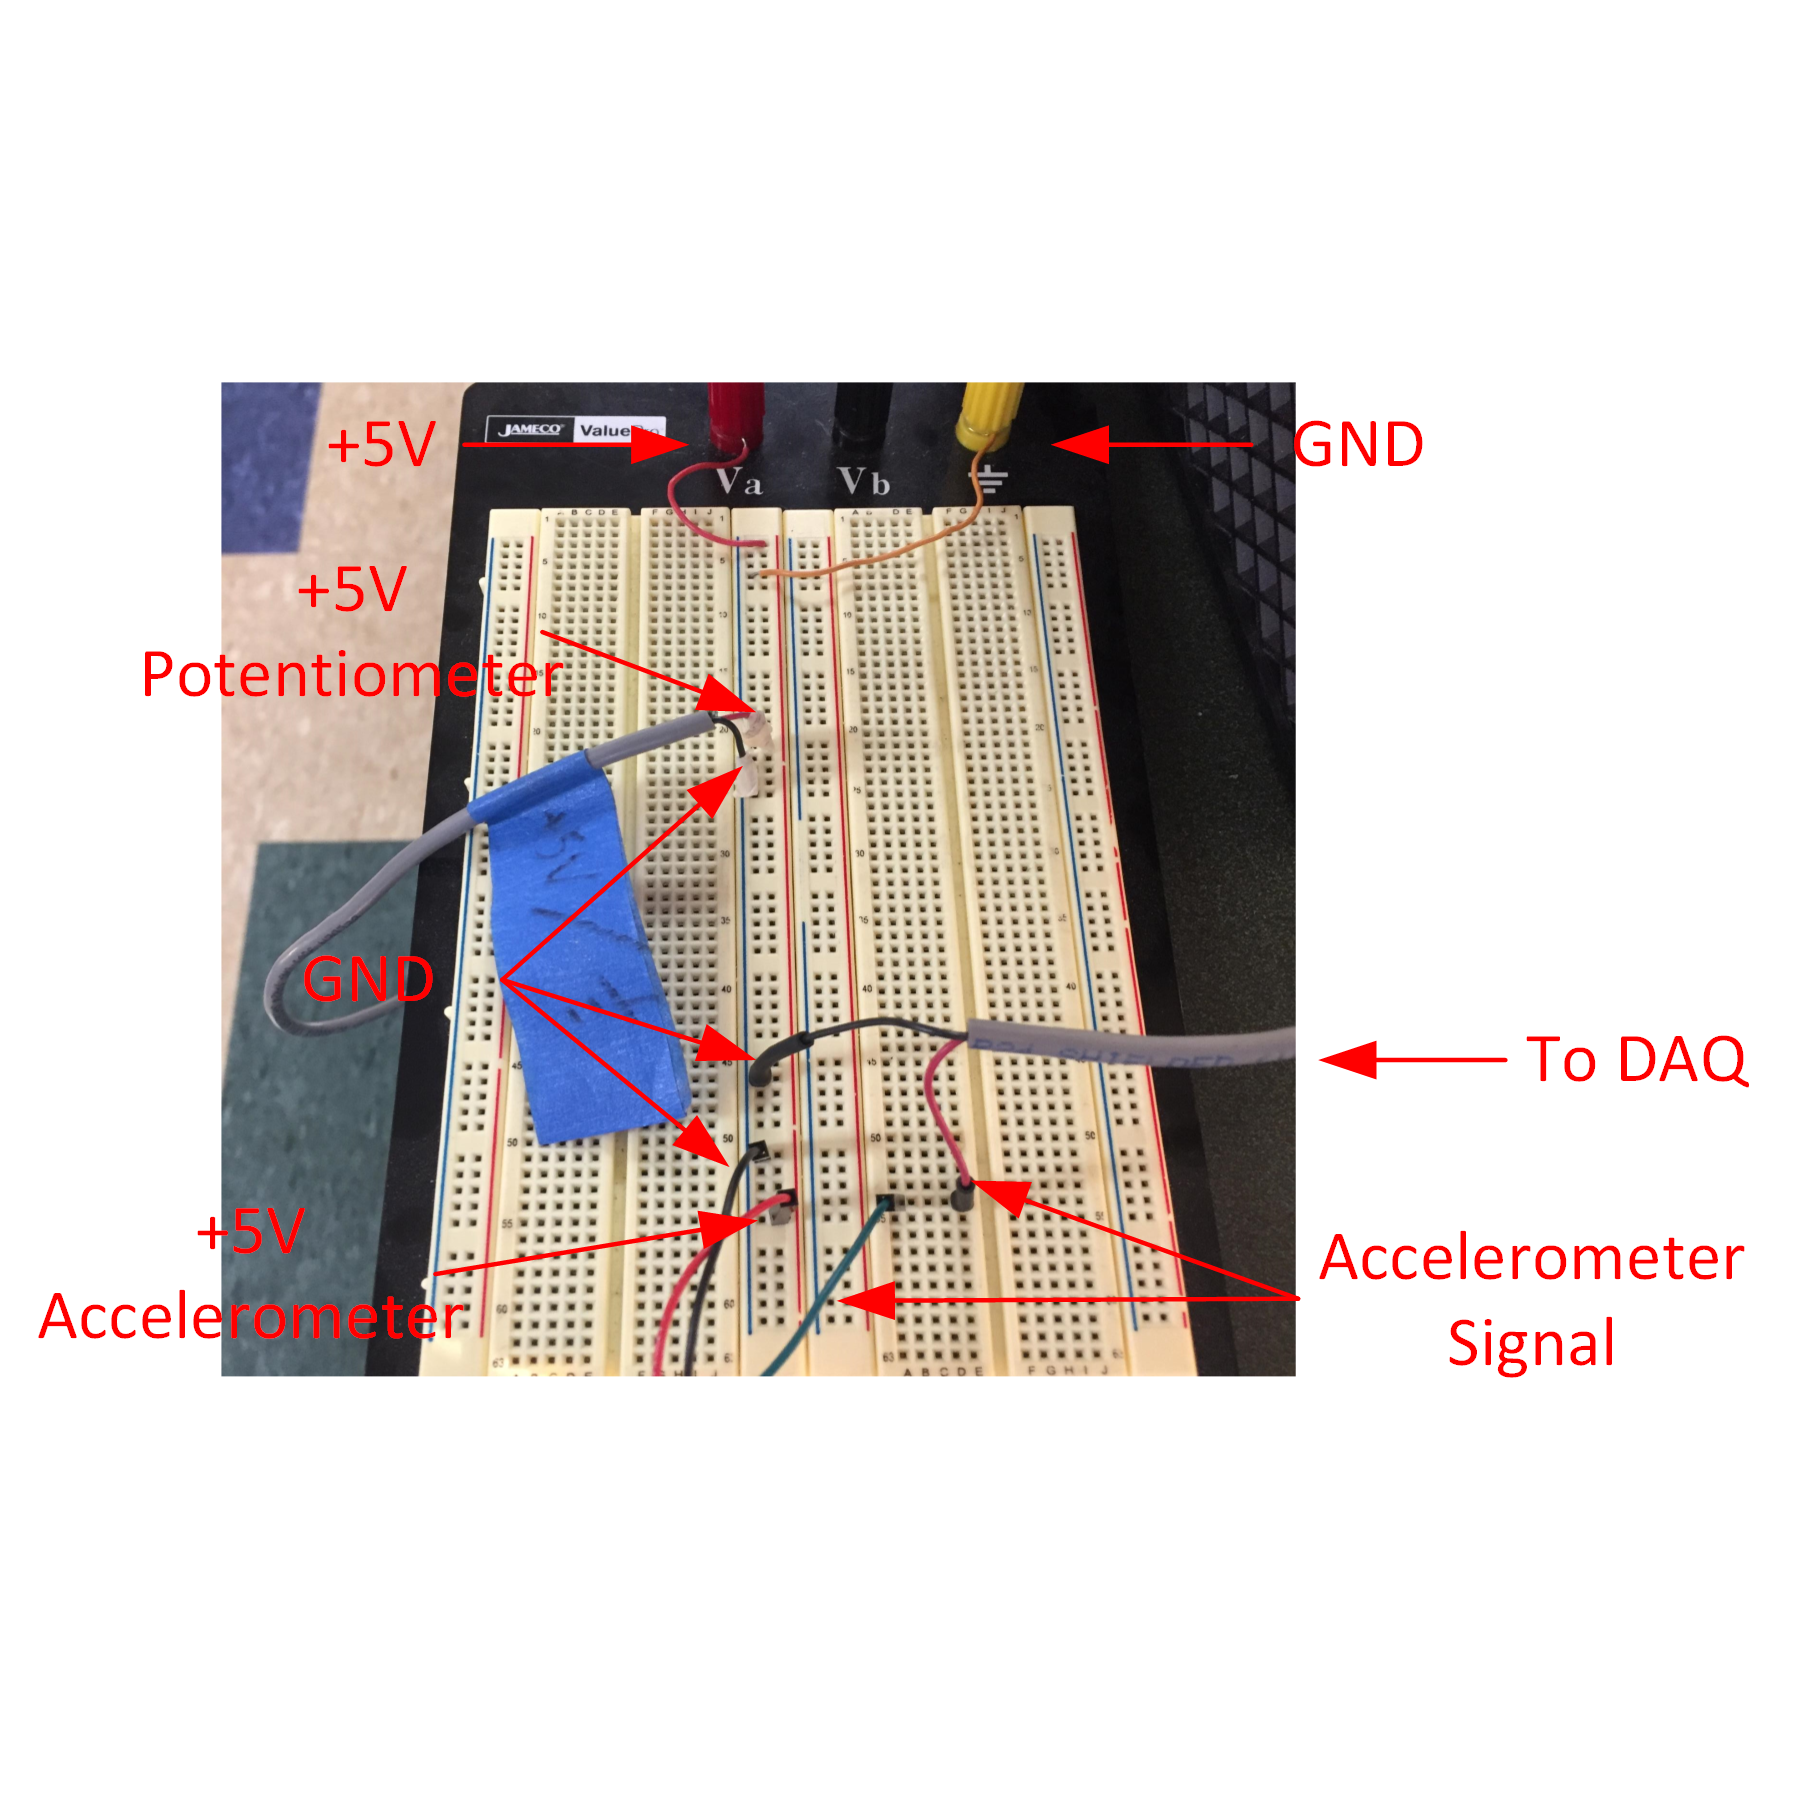
\includegraphics[width=3.0in]{Lab03Fig02.png}}%
\end{figure}

\begin{figure}[!ht]
\centering
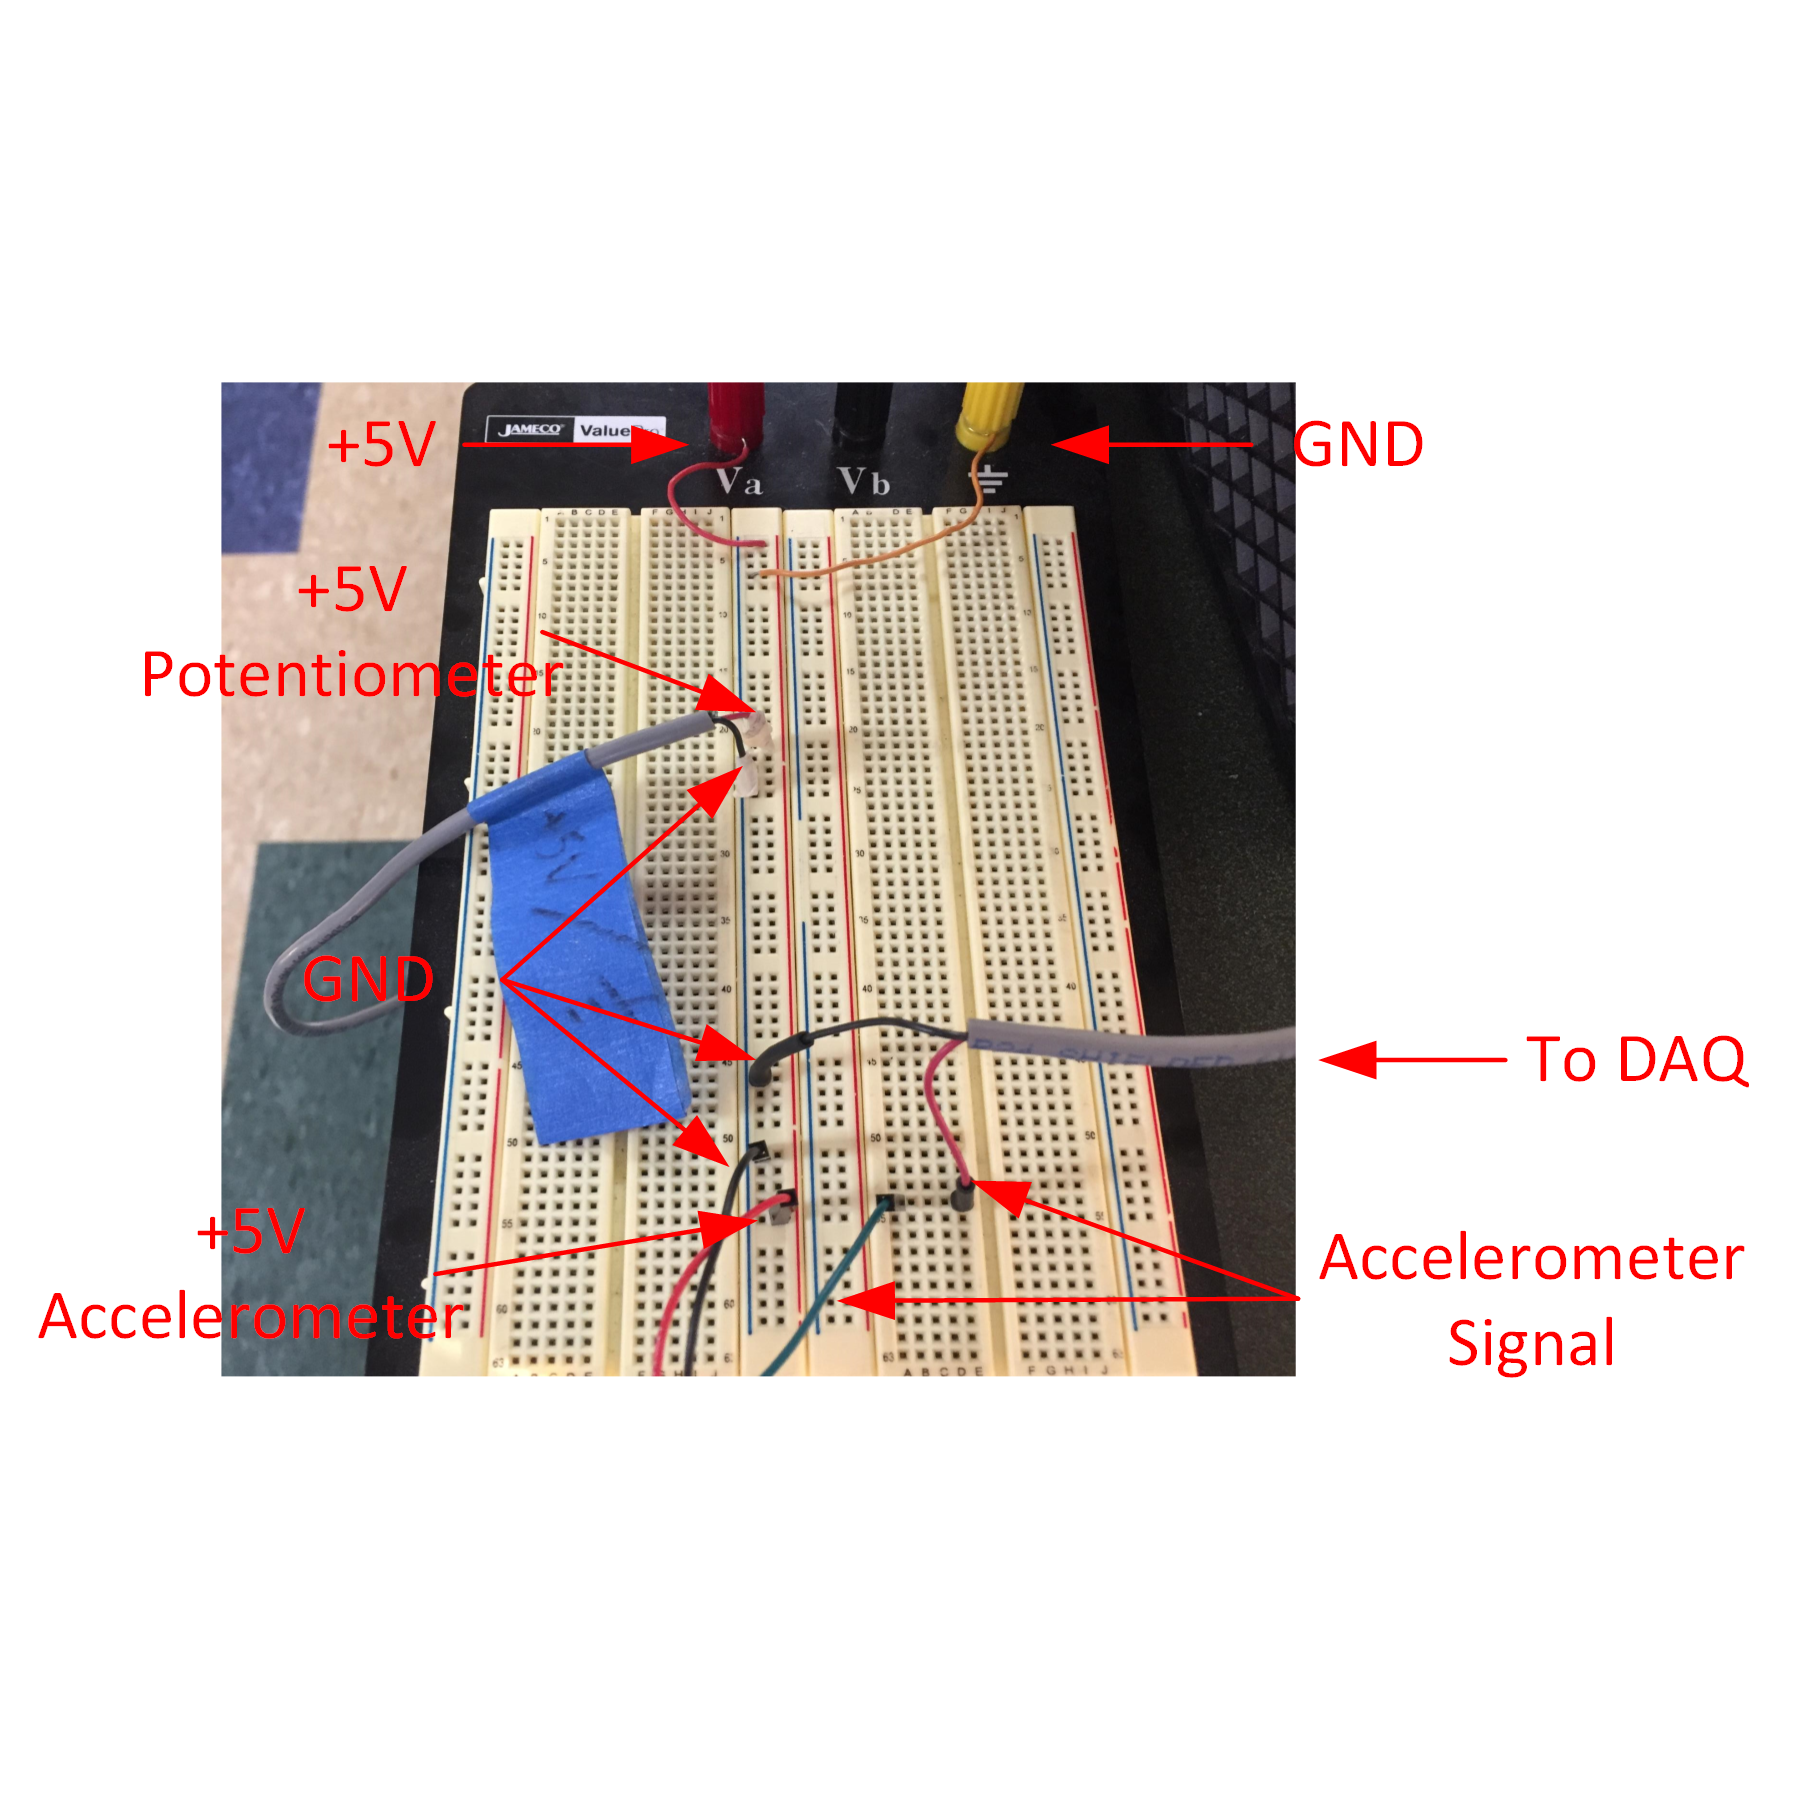
\includegraphics[width=3.00in]{Lab03Fig02.png}
\caption{Connection to the NI-DAQ system.}
\label{fig:fig03C}
\end{figure}
\clearpage
\section{Part-C}
Test your acquisition program and test data acquisition system
\begin{itemize}
\item Make sure that you are acquiring two channels of data from DAQ system
\item When you have verified your circuit and connections, run your Matlab program.
\item Modify the calibration bias as necessary to zero the pendulum as is hangs at the bottom.
\item Confirm that you are acquiring data from the accelerometer. You will need the y-axis accelerometer
voltages for the calibration step that follows (Part-D).
\end{itemize}


\section{Part-D}
Calibrate the y-axis accelerometer outputs.
\begin{itemize}
\item Complete the table below in your logbook by rotating the pendulum to the four shown positions and recording the output voltages on the y-axis of the accelerometer. Collect the voltage output from accelerometer for 20 seconds at a sampling rate of 20Hz. Make sure that you have saved these calibration file, if you need to verify your calibration. Fill the information in the table provided below.
\item Plot the data points from the above table in order to create calibration equations for the y-axis acceleration measurements. Specifically, Plot $ay_g$ vs. $ay_{v,avg}$ to find y-axis acceleration (in $m/s^2$) as a function of sensor voltage.
\end{itemize}
\begin{table}[!hb]
\centering
\caption{Sample calibration data for experiment 2.}
\begin{tabular}{c|c c c}
\toprule
Pendulum & & y-axis acceleration & Average output voltage  \\
orientation &Schematic &$ay_{g}$ ($m/s^2$) & $ay_{v,avg}$ (v) \\ \toprule
Right& 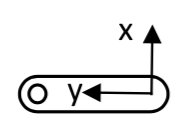
\includegraphics[width=0.40in]{Fig03A} & 0.00 & \\ \hline
Up   & 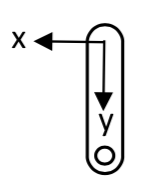
\includegraphics[width=0.30in]{Fig03B} & 9.81 & \\ \hline
Left & 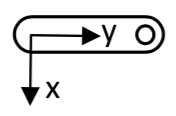
\includegraphics[width=0.35in]{Fig03D} & 0.00 & \\ \hline
Down & 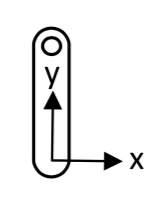
\includegraphics[width=0.35in]{Fig03C} &-9.81& \\
\bottomrule
\end{tabular}
\end{table}


\section{Part-E}
\emph {Now add your calibration equation to acquisition program to display the pendulum angle in degrees during the data acquisition process and acceleration values in $m/s^2$. }
\begin{itemize}
\item You will have to change the slope and intercept values in the provided Matlab program.
\item Run your Matlab program for few seconds and see if your program displays the correct angle and acceleration values.
\item Show your program and results to the TAs to verify your program. {\bf If program is working properly, the proceed to collect data.}
\end{itemize}

\section{Part-F}
\emph {Procedure for collecting data}
\begin{itemize}
\item Change the sampling rate to 500 hz and sampling time to 15 seconds. Use the code provide in section \ref{app:acqCode}.
\item Make sure the output file is named as ``Expt\_03\_FirstName\_Lastname.dat''
\item Make sure to input the appropriate slope and intercept values to convert voltage data from potentiometer to angles in degrees and voltage from accelerometer to acceleration.
\item Move the pendulum the horizontal position location.
\item Start the acquisition program 
\item Release the pendulum 
\item Make sure the plot shows pendulum angular location and pendulum normal acceleration.
\item Show the final output figure to the TAs.
\item Open your output file and check the data. 
\item Output file should have three columns of data. The first column will have time information, second column will have angular position of pendulum in degrees, and the third column will have acceleration value from accelerometer in $m/s^2$.
\end{itemize}

\section{Part-G}
\emph{Post processing of the data}
\begin{itemize}
\item Open the file using Matlab program and read all three columns of data.
\item Convert the angle value in radians
\item Remove the acceleration due to gravity from the accelerometer data
\begin{itemize}
\item Here you have to use free-body diagram to identify the contribution from acceleration due to gravity
\item Use the angular value for pendulum to accurately identify the position of the pendulum.
\item The result will be the measured normal acceleration of the pendulum due to angular velocity.
\end{itemize}
\item Plot the normal acceleration data from accelerometer and normal acceleration using equation \ref{Eq:NormAcc} in a single plot. 
\item Plotting the noisiest data first (This way the other data will remain visible). Sample plot is shown in Figure \ref{fig:postPr}.
\item Code to create post-process file is shown in appendix \ref{app:plotAccData}
\end{itemize}
\begin{figure}
\centering
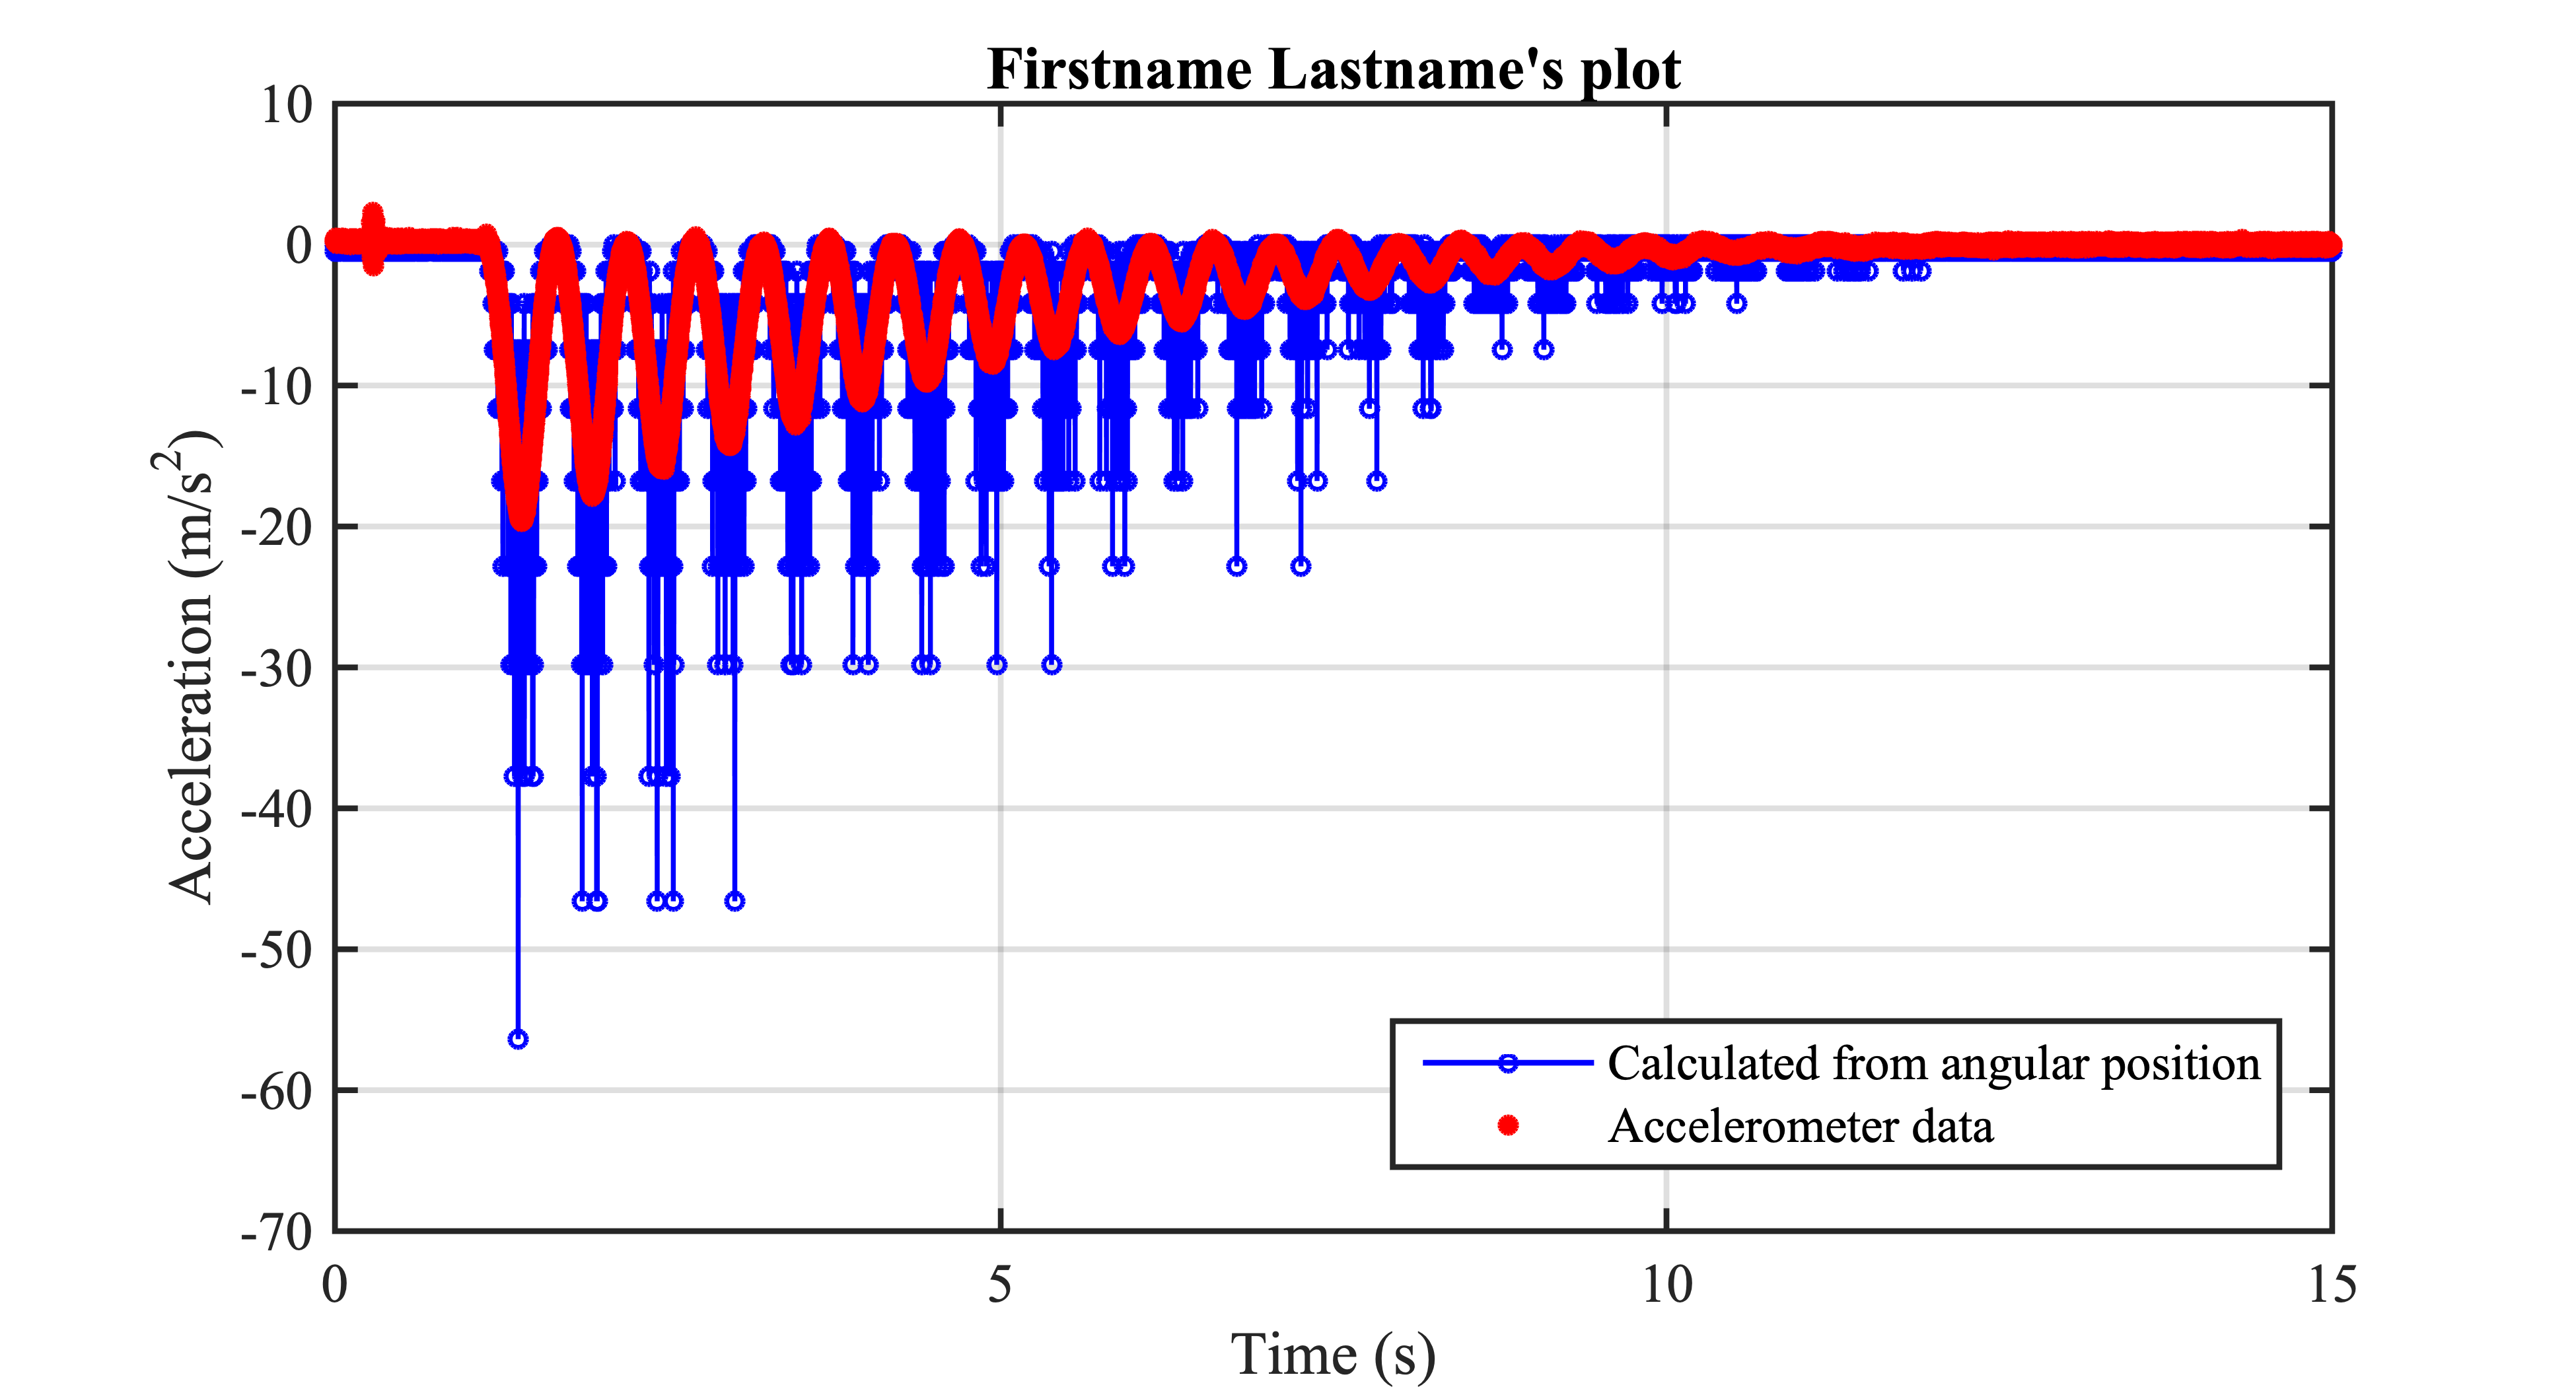
\includegraphics[width=6.00in]{Firstname_Lastname_Expt02_Postprocess.png}
\caption{Sample post-process plot.}
\label{fig:postPr}
\end{figure}

\section{Part-H}
Return lab space to prior condition
\begin{itemize}
\item Turn off the power supply.
\item Remove wires connecting the power supply to the breadboard and return to the wall
\item Remove all breadboard wires and place them back in the wire kit in an organized fashion.
\item Remove the pendulum wires from the breadboard and set aside.
\item Log off the computer.
\item Make sure to copy the data to your harddrive.
\item {\bf Do this for every lab!}
\end{itemize}


\section{Instruction}
\begin{itemize}
\item Make sure to name the files your FirstName\_ LastName\_ QuestionNumber, use the format provided in the sample Matlab code. Make sure the submitted figure has the title. Include the apostrophe!
\item Make sure to submit your post-lab assignment on the BBLearn website. 
\item Here are some details to help. 
\begin{itemize}
\item Plot  the experimental data using red circles with MarkerSize 8. Experimental data points should always be plotted using markers without lines connecting the points
\item Plot curve from theory (or curve fit line) using a solid colored line with LineWidth 2. 
\item  Set the x and y-axis limits for each figures. Follow the instruction.
\item Make sure the major grid lines are visible
\item All plot text should be in Times font. You will need to specify this for the title, labels, and
legends. The axis labels and numbers should be in 10-point font
\item The title should be in 10-point font
\item Make sure to add the legend. Keep in mind that legend should not hide the plotted data
\item For full credit make sure that your submitted files look similar to the sample figures shown in the document
\item All the submitted plot should be in png format with 600 dpi resolution.
\item If in doubt make sure to request the TAs for help
\end{itemize}
\end{itemize}

\section{Post lab (50 points)}
\textbf {Postlab are due at Friday 5:00 pm.} For this experiment submit the following items on BbLearn for your post-laboratory assessment.
\begin{enumerate}
\item Accelerometer Calibration Plot. Submit a calibration plot showing the raw data points as markers and the calibration curve as a line. The plot should be 6.5inch wide. Make sure to properly annotate your plots: axis labels, titles, legend, etc. Using the text command in Matlab, place the equations or numbers listed below on the plot. Use Greek symbols where appropriate.
\begin{enumerate}
\item The calibration equation on the plot with 4 significant digits for each number. 
\item The norm of the residuals of your linear regression.
\item The standard error of the fit for your calibration equation (Make sure to include appropriate units.)
\end{enumerate}
\item Pendulum Swing Plot. Submit a time series plot showing normal acceleration vs. time calculated in
the two ways described in Part-G.
\begin{enumerate}
\item Normal acceleration measured from the accelerometer vs. time.
\item Normal acceleration calculated from the equation $a_n = \dot{\theta}^2r$ .
\item The plot should be 6.5inch wide. Make sure to properly annotate your plots: axis labels, titles, legend, etc. Use Greek symbols where appropriate.
\end{enumerate}
\item Answer all question in the post-lab assessment on BbLearn
\end{enumerate}


%-----------------------------------------
%\clearpage
%\section{Appendix}
%Sample code for data acquisition using Matlab
%\lstinputlisting{../MatlabProgram/mainAcqProgram-NousMacBookPro.m}
%\clearpage
%\lstinputlisting{../MatlabProgram/plotAndLogData.m}
%\clearpage

\clearpage
\section{Appendix}
%\subsection{Matlab program to test the circuit}
%\label{app:testingCode}
%\lstinputlisting{../MatlabProgram/Ver01/mainAcqProgram_ForTesting.m}
%\clearpage

\subsection{Matlab program to acquire data for calibration}
\label{app:calibCode}
\lstinputlisting{../MatlabProgram/Ver01/mainAcqProgram_ForCalibration.m}

\clearpage
\subsection{Matlab program to generate calibration plot}
\label{app:genCalib}
\lstinputlisting{../MatlabProgram/Ver01/generate_CalibrationPlot.m}

\clearpage
\subsection{Matlab program to acquire data}
\label{app:acqCode}
\lstinputlisting{../MatlabProgram/Ver01/mainAcqProgram_ForCollectingData.m}

\clearpage
\subsection{Matlab program to plot acceleration data}
\label{app:plotAccData}
\lstinputlisting{../MatlabProgram/Ver01/Rodrigo_Padilla_Exp03_PostProcess.m}

\end{document}